\begin{abstract}
In this paper, we examine the impact of 3 different loss functions, used as an objective function, when training models with x-vector architecture. X-vector architecture is deep neural network (DNN) architecture, whose main goal is to extract distinctive representations of a speakers from speaker utterances. Extracted representations of speakers from x-vector architecture are high dimensional vectors called x-vectors. Although x-vector architecture is implemented in some publicly available frameworks, we have worked with our own pytorch implementation. In~the project, we have evaluated the trained models with a speaker verification metric: equal error rate (EER). As a backend, to compare pairs of x-vectors,  we have used cosine similarity. Performance of the x-vector model was the best, when we used, as an objective function for the training model, our own implementation of Angular Softmax Loss ($EER= 8.04 \%$) . On the other hand, performance was the worst, when we used pytorch implementation of Triplet Margin Loss ($EER=16.46 \%$). Details, why the Triplet loss function failed are described further in paper.
\end{abstract}

\section{Introduction}

Machine learning tasks connected with audio (speaker verification, speaker identification) had for a really long time a good performing basis in statistical models called Gaussian Mixture Models (GMM) \cite{gmm}. Significant performance improvement over GMM came with vector representations of speakers called i-vectors (i-vectors are vectors produced by Joint Factor Analysis over GMM mean supervectors) \cite{i_vectors}. In~the project, we have worked with vector representations of speakers called x-vectors. Using x-vectors, for speaker verification or identification, is not a state of the art approach anymore, but they offer more discriminative abilities between different speakers than i-vectors \cite{x_vectors}. 

\medskip

For producing x-vectors, we have used DNN architecture, which is shown in figure \ref{fig:x-vectors_architecture}. Most interesting part of architecture, statistical pooling layer, is located between convolution and fully connected layers. This layer is necessary for producing speaker embeddings from variable-length utterances. Statistical pooling layer aggregates frame-level information into one embedding by joining mean and standard deviation of outputs from convolution layers. Networks with this architecture can be simply trained to correctly classify speakers from a training dataset with multiclass Cross entropy as an objective function (see \ref{simple_softmax_training}). This way model learns how to extract discriminative features from variable length utterances of speakers. After training of the model, any speaker utterance can be passed as input to the model and outputs from the first or second fully connected layer, are desired x-vectors. Authors of architecture, in~their experiments,  find out, that better results for speaker verification give x-vectors, which are output from first fully connected layer \cite{x_vectors}.


\begin{figure}[h]
    \centering
    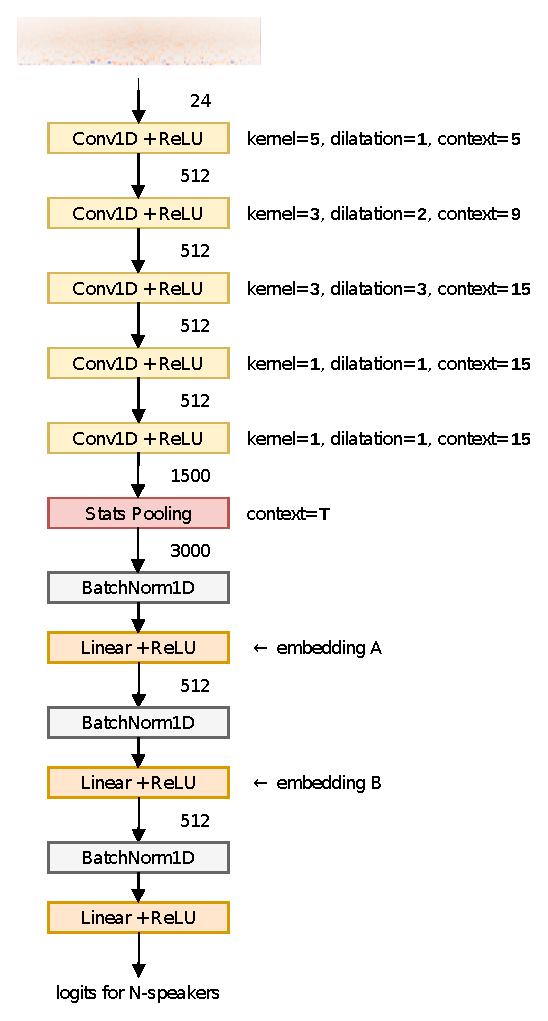
\includegraphics[height=0.5\textwidth]{x-vectors-diag.eps}
    \caption{DNN architecture for extracting x-vectors}
    \label{fig:x-vectors_architecture}
\end{figure}
